
\setchapterpreamble[ur][.6\textwidth]{%
\dictum[Umberto Eco, \textit{The Name of the Rose} (1954)]{%
``Then why do you want to know?''\\
``Because learning does not consist only of knowing what we must or we can do, but also of knowing what we could do and perhaps should not do.''
}\vskip1em
} 


\chapter[Evolution or plasticity?]{Disentangling evolutionary, plastic and demographic processes underlying trait dynamics: A review of four frameworks}

Koen J. van Benthem*, Marjolein Bruijning*, \textbf{Timoth\'ee Bonnet}*, Eelke Jongejans$^\dagger$,
Erik Postma$^\dagger$, Arpat Ozgul$^\dagger$
\begin{itemize}
\item[*] co-first authors
\item[$\dagger$] co-last authors
\end{itemize}

\section{abstract}
\noindent \begin{enumerate}
\item Biologists are increasingly interested in decomposing trait dynamics into underlying processes, such as evolution, plasticity and demography. Four important frameworks that allow for such a decomposition are the quantitative genetic animal model (AM), the `Geber' method (GM), the age-structured Price equation (APE), and the integral projection model (IPM). However, as these frameworks have largely been developed independently, they differ in the assumptions they make, the data they require, as well as their outcomes and interpretation. 
\item Here we evaluate the way each of these frameworks decompose trait dynamics into underlying processes. To do so, we apply them to simulated data for a hypothetical animal population. We simulated scenarios with and without selection on body size, and with high and low heritability. In all four scenarios, body size also contained a plastic component.
\item The APE and IPM provided similar results, as did the AM and GM, with important differences between the former and the latter. All frameworks detected positive contributions of selection in the high but not in the low selection scenario. However, the APE and IPM did not distinguish between the high and low heritability scenarios, while the AM and GM did. Both the AM and GM revealed a high contribution of plasticity. In all scenarios, the APE and IPM attributed most of the change in body size to ontogenetic growth and inheritance, which include the effects of plasticity, maternal effects and heritability. We show how these apparent discrepancies are mostly due to the aims and definitions of the different frameworks. For example, the APE and IPM capture selection, whereas the AM and GM focus on the response to selection. Furthermore, the frameworks differ in the processes that are ascribed to plasticity and to their method for taking into account demography.
\item We conclude that because of the inherent differences among frameworks, no single framework provides the `true' contributions of evolution, plasticity and demography. However, with a thorough understanding of any of these frameworks, they will provide valuable biological insight. This work thus supports both future analysis as well as the careful interpretation of existing work.

\end{enumerate}

\section{Introduction}

%%%%%%%%%%%%%%%%%%%%%%%%%%%%%%%%%%%%%%%%%%%%%%%%%%%%%%%%%%%%%%%%%%%%%%%%%%%%%%

Understanding trait and population dynamics and how the two are intertwined is crucial for predicting population resilience and viability \parencite[e.g.][]{merila2014}. Hence, which processes shape population-level trait dynamics (i.e., changes in trait distributions over time) is a fundamental question in ecology and evolution, and one which is gaining in urgency given mounting concern regarding the consequences of anthropogenic environmental change for natural populations \parencite[e.g.][]{parmesan2006}.

Phenotypic trait distributions may be altered across generations by genetic (i.e. evolutionary) processes, as well as by non-genetic processes, such as phenotypic plasticity. Since the realisation that evolutionary and ecological processes may act on the same time scale, distinguishing between the role of evolution and plasticity has been the subject of a substantial body of research \parencite{Hairston2005,Gienapp2008,Post2009}. To complicate matters further, changes in the demographic structure of a population may additionally shape trait distributions \parencite{Coulson2008}. Hence, understanding and predicting trait dynamics ideally requires simultaneously taking into account all three processes \parencite{Pelletier2007,Schoener2011}. 

To date, four major frameworks aiming at distinguishing between the role of evolution, phenotypic plasticity and demography have been developed: 1) The quantitative genetic framework, particularly the animal model \parencite[AM; e.g.][]{Henderson1950}, 2) the `Geber method' \parencite[GM;][]{Hairston2005}, 3) the age-structured Price equation \parencite[APE;][]{Coulson2008}, and 4) the application of the APE in conjunction with an integral projection model \parencite[IPM;][]{easterling2000,Ellner2006,Coulson2010}. As of yet, several studies have tried to explicitly estimate the relative importance of evolution, plasticity and/or demography using one of these approaches \parencite[e.g.][]{Reale2003, Ezard2009, Ozgul2009, Rebke2010, Becks2012, Morrissey2012b}. Nevertheless, fully disentangling and quantifying evolutionary, ecological and demographic processes and thereby predicting the consequential trait dynamics has proven to be problematic \parencite{Gienapp2008,Schoener2011,merila2014}. At least some of these difficulties can be attributed to the large amounts of (individual-based) long-term data required, which are often unavailable for natural populations \parencite{Clutton-brock2010}. However, even if sufficient data are available, synthesis of the results from the four frameworks is hampered by the fact that they have been developed largely independently of each other. As a consequence, they differ in their focus and aims, and as we show here, they define biological processes in non-equivalent ways.  

Here we provide a comparison of the differences, similarities and complementarity of each of these four decomposition frameworks by applying them to the same simulated datasets and comparing their outcomes. Thereby, we evaluate how they quantify the role of different ecological and evolutionary mechanisms in shaping trait dynamics under a range of biological scenarios. Together with a critical review of the theory underlying each of the frameworks, we provide comprehensive insight into their underlying assumptions, as well as the conceptual differences and similarities. This provides a much needed overview of the suitability of each framework with respect to both research questions and data availability.

%%%%%%%%%%%%%%%%%%%%%%%%%%%%%%%%%%%%%%%%%%%%%%%%%%%%%%%%%%%%%%%%%%%%%%%%%%%%%%


\section{Applying the four frameworks}

%%%%%%%%%%%%%%%%%%%%%%%%%%%%%%%%%%%%%%%%%%%%%%%%%%%%%%%%%%%%%%%%%%%%%%%%%%%%%%

\subsection{Data simulation}

Although it comes with the loss of some biological realism, using simulated rather than empirical data enables us to evaluate the frameworks under different scenarios and allows for replication. Furthermore, it ensures perfect knowledge of the processes that shape trait dynamics, acting as a reference against which to compare the results of each framework. Finally, simulated data do not suffer from the complications introduced by missing data. 

Data were simulated using a two-sex individual-based model of a closed population of a hypothetical animal species, implemented in R \parencite{R}. Here, we provide a brief overview, while a more complete description can be found in SI \ref{app:simul}. We also provide the R code on \newline \verb|https://github.com/koenvanbenthem/Disentangling_Dynamics_IBM|. We simulated a single trait, body size $z$. Size at birth is determined by an individual's genotype (10 loci, with 10 alleles each and mendelian inheritance, more details in SI \ref{app:simul:gen}), the body size of its mother, and a stochastic component (drawn from a Gaussian distribution; SI \ref{app:simul:birth}). Ontogenetic growth results in an increase of body size with age. Growth rate is proportional to body size and decreases with age, and is further influenced by per-capita food availability (SI \ref{app:simul:growth}). Males were randomly assigned to females, who have a $50\%$ chance of becoming reproductive after one year and whose reproductive probability increases with age. The litter size that a female produces depends on per-capita food availability, a stochastic component, and body size (SI \ref{app:simul:repr}). Survival probability first increases with age, but starts decreasing after year five, reflecting senescence, and is further influenced by per-capita food availability and body size. Maximum age is 30 years. Furthermore, a trade-off exists between female reproduction and survival, i.e. reproducing at time $t$ decreases survival probability to time $t+1$ (SI \ref{app:simul:surv}). 

Fifty time steps were simulated, of which the first ten were discarded from further analyses to allow the age structure to stabilize (Fig. \ref{simdata:6}). After ten years, total food availability started to decline. As food is divided over all individuals alive in a given year, with some individuals randomly obtaining more than others, the decline affects population and trait dynamics through individual survival, growth and (female) reproductive success (SI \ref{app:simul:food}). The remaining data spanned 40 years (i.e. approximately 13 generations), which is comparable to the length of some of the field studies these frameworks have been applied to \parencite{Clutton-brock2010}. 

To evaluate the behaviour of the frameworks under different circumstances, we simulated four different scenarios. First, survival and fertility selection on body size was either present ($s_+$) or absent ($s_0$). Under the $s_+$ scenarios, there was a positive effect of body mass on survival and on litter size for mothers. Second, the relative importance of genetic variation in shaping body size, commonly measured as heritability, was either high ($h_+$) or low ($h_-$). This was done by using either of two pre-defined genotype-phenotype maps: one with big and one with small variation in the effects of alleles. Furthermore, the plastic component in birth size was varied antagonistically. The parameter values for each of the four scenarios (\sh, \sH, \Sh and \SH) can be found in SI \ref{app:scenarios}. To evaluate the effect of stochasticity, each scenario was replicated 100 times.

Figure \ref{simdata} provides an illustration of some of the key characteristics of the datasets simulated under each scenario. Despite a substantial amount of stochastic variation across replicates within each scenario, clear differences in trait and population dynamics are apparent. As expected, the $s_+$ scenarios show a positive relation between body size and annual fitness, calculated as the sum of the survival and litter size to $t+1$, whereas the $s_0$ scenarios do not (Fig. \ref{simdata:4}). Furthermore, the proportion of the phenotypic variance attributable to variance in the simulated genotypic values (i.e. broad-sense heritability $\text{H}^2$) was ca. 0.50 in the $h_+$ and 0.08 in the $h_-$ scenario.

Although in all scenarios population size first increased (until year 20) and then decreased (Fig. \ref{simdata:1}), the  population size averaged across replicates reached up to 322 and 334 individuals in scenarios \Sh and \SH, whereas in \sh and \sH the maximum average population size was 245 and 252 individuals, respectively. Mean body size first increased rapidly, but started to decrease in all scenarios after the tenth year (Fig. \ref{simdata:2}): in \sh with \Range{-0.47}{-1.45}{0.63 \; 95\% \; \text{range among replicates}}, in \sH with \Range{-0.46}{-1.59}{0.0.68}, in \Sh with \Range{-0.75}{-1.87}{0.08}, and in \SH with \Range{-0.16}{-1.12}{0.83}.

Genotypic values for birth size, however, continued to increase only in scenario \SH, whereby the change was \Range{0.62}{0.23}{1.04} (Fig. \ref{simdata:3}). In \Sh a smaller increase was observed \Range{0.08}{-0.074}{0.24}, whereas \sh and \sH show on average no change in genotypic values. Correspondingly, average birth size increased only in the \SH scenario, with \Range{0.58}{0.092}{1.11}, between year 11 and year 50 (Fig. \ref{simdata:5}). 

%%%%%%%%%%%%%%%%%%%%%%%%%%%%%%%%%%%%%%%%%%%%%%%%%%%%%%%%%%%%%%%%%%%%%%%%%%%%%%


%%%%%%%%%%%%%%%%%%%%%%%%%%%%%%%%%%%%%%%%%%%%%%%%%%%%%%%%%%%%%%%%%%%%%%%%%%%%%%%%%%%%
%%%%% OVERVIEW OF THE FRAMEWORKS AND THEIR APPLICATION
%%%%%%%%%%%%%%%%%%%%%%%%%%%%%%%%%%%%%%%%%%%%%%%%%%%%%%%%%%%%%%%%%%%%%%%%%%%%%%%%%%%%
%%%%%%%%%%%%%%%%%%%%%%%%%%%%%%%%%%%%%%%%%%%%%%%%%%%%%%%%%%%%%%%%%%%%%%%%%%%%%%

\subsection{Decomposing simulated trait dynamics}
%%%%%%%%%%%%%%%%%%%%%%%%%%%%%%%%%%%%%%%%%%%%%%%%%%%%%%%%%%%%%%%%%%%%%%%%%%%%%%
Rather than providing an exhaustive overview of all methods allowing for the decomposition of trait dynamics, we have chosen to focus on four, commonly-used frameworks. The four frameworks have different data requirements (see Fig. \ref{overview} for a schematic overview) and do not yield identical results. This is illustrated in the following section, in which we analyse the simulated data using each of the frameworks.

\paragraph{Animal Model} 
%%% GENERAL ABOUT THE AM
The animal model (AM) is a quantitative genetic method that was developed for commercial breeding \parencite{Henderson1950,Henderson1976}, where it has been used successfully for several decades \parencite[e.g.][]{Lynch1998}. Only recently has it been applied to wild animal populations \parencite[e.g.][]{reale2003,Postma2014} and plant \parencite{Stinchcombe2014} populations. For extensive explanations of the AM as applied to natural populations, see \cite{Kruuk2004} and \cite{Wilson2009}. 

The AM is a linear mixed effects model that is fitted to individual-level data. The variance in a phenotypic trait ($z$) is partitioned into genetic and non-genetic sources of variation. Under the assumption that this partitioning is additive (i.e. in the absence of genotype-environment correlations and interactions), $z$ can be written as the sum of a population mean ($\mu$), an additive genetic effect (the breeding value, $a$) and a residual (environmental) value capturing plasticity ($e$), thus $z=\mu+a+e$. Information on the relatedness between individuals (estimated from a pedigree or genetic markers) is used as a constraint in the fit, allowing for the estimation of $a$. If the data allow for it, other components contributing to variation in $z$, such as maternal, common, and permanent environmental effects can be accounted for explicitly. This variance decomposition can be used to predict response to selection on the long-term, assuming a quantitative genetic model, where ideally an infinity of genes contributes to phenotypic variation so that the distribution of effects is Gaussian. In practice, four or five bi-allelic genes are sufficient \parencite{Roff2007}.

There are several ways to estimate evolution within the AM framework (see discussion), but here we illustrate only one of these. We fitted a univariate AM and quantified the change in the best linear unbiased predictors (BLUPs) for the breeding values over time \parencite[][and references therein]{Postma2006,Hadfield2010}. We used body size as the sole response variable, and intercepts for breeding values, maternal effects, permanent environment effects, and year effects were included as random effect. Maternal and permanent environment effects were modelled by fitting maternal and individual identity, respectively. Age was included as a continuous fixed effect (both as linear and quadratic terms). All fits were performed using the R-package \texttt{MCMCglmm} \parencite{Hadfield2010}. The posterior distributions were estimated based on 1,000 MCMC samples, from 50,000 iterations with a thinning interval of 40 and a burn-in of 10,000, thus maintaining the correlation between successive samples of all parameters below 10\%. 

We estimated the temporal trend in the BLUPs for all random effects. We accounted for their uncertainty following \cite{Hadfield2010b} by performing a regression of the BLUPs on time for each MCMC sample of the model. This provided a posterior distribution of linear slope coefficients, estimating the change in additive genetic, maternal, and permanent environment effects per time step. More details on the fitted models are given in SI \ref{app:am:blup}.

As depicted in Figure \ref{frameworkresults:2}, in all scenarios the contributions of evolution and individual plasticity were largest, while the contributions of permanent environment and maternal effects were very small. On average, we found positive changes in breeding values in both scenario \Sh  (\Range{0.0013}{-0.0038}{0.0095} and scenario \SH \Range{0.014}{0.00021}{0.029}. Note that genetic drift introduces a substantial amount of variation in the rate of evolutionary change among replicates in the $h_+$ scenario, which is reflected in the large error bars in Fig. \ref{frameworkresults:2}). Negative contributions of individual plasticity were found, particularly in the scenarios with selection \Range{-0.02}{-0.049}{0.0018} and \Range{-0.019}{-0.045}{0.0029} for $h_{-}$ and $h_+$, respectively.

In the $s_0$ scenarios, although drift generates variation around the mean contribution of evolution, we would expect the latter to be 0. However, our model inferred  a genetic decline for $h_{-}$ and $h_+$ in the scenarios without selection \Range{-0.0057}{-0.016}{0.0040} and \Range{-0.0073}{-0.024}{0.0087}, respectively.
 This pattern was confirmed by the genetic values we simulated. The AM therefore estimates evolution with a negative bias. The reason seems to be that we fit a model not matching the simulation process. As mean size decreases with time, the contributions of mothers to birth size decreased too. Maternal effects are modelled as maternal identity rather than maternal current size, however, and the AM incorporates this change in the evolution term. 
% But when the genotypic values are decreasing as well, this would mean that decline is real rather than an artefact of not fitting the right model. Isn't what you are seeing evolution of the maternal size? I don't think you would ever expect to pick up such an effect by looking at the change maternal blups. 
% TK: Genotypic values were not actually declining in these cases. The current GM figure is a propagation of the AM results and no longer reflects actual genotypic values. These are shown in the GM appendix and show no change on average for the 0-selection scenario. Furthermore we think that if the quality of mothers is allowed to change over time, this should be captured in the BLUPs. 

% Related to the above, I am not sure how interesting it is to look at changes in the permanent environment effect. Which process do they capture? In my experience pe effects tend to confuse people, especially if you don't very carefully define them. I agree that they should be included in the model to obtain better estimates of genetic and environmental change, but not sure if they should be included in the figure.
% TK: We would say that it should capture changes in the plasticity in birth size, which did not vary over time in the model and this is also reflected in the numbers (fig. 3). Furthermore, we would like to include, evne if just for completeness, but also because maybe they are not very interesting here, we want to give people a grip on these frameworks and hence we should discuss all terms. 
\paragraph{Geber method}
%%% GENERAL DESCRIPTION GM
The `Geber method' (GM) \parencite{Hairston2005} is a very general method that quantifies how temporal changes in various factors influence the response variable of interest. The biological assumptions vary with the specific factors and response variable. It may for example estimate how temporal changes in mean breeding value $\overline{a}$ and in an environmental factor $k$ such as food availability propagate to a population-level response variable $X$, such as mean trait value. Examples of its application can be found in \cite{Ellner2011} and \cite{Becks2012}.

%%% OUR APPLICATION OF THE GM
For the implementation of the GM, we followed the analysis of fledgling mass of great tits in \cite{Ellner2011}. Here, the average body size is taken as the population-level response variable. The change in mean trait ($\overline z$) in the simulated populations was decomposed into a contribution of the environment ($\overline k$) and a contribution of a phenotypic change in size at birth. The latter was decomposed further into an evolutionary ($\overline a$) and a plastic component ($\overline p$):

\begin{equation}
\frac{d \overline{z}}{dt} = \frac{\partial \overline{z}}{\partial \overline{k}} \frac{d\overline{k}}{dt} + \frac{\partial \overline{z}}{\partial \overline{a}}\frac{d \overline{a}}{dt} + \frac{\partial \overline{z}}{\partial \overline{p}}\frac{d\overline{p}}{dt} 
\end{equation}

For each year between years 11 and 50, we calculated the mean body size ($\overline z$), mean size at birth of newborns, the average food availability that alive individuals had access to during their lifetime up to that moment ($\overline k$), and the mean breeding value as estimated by the AM ($\overline a$) (see above). Hence, as breeding values are typically not observed directly, the application of the GM to empirical data relies on other methods such as the AM for their estimation. Finally, we calculated a plasticity term ($\overline p$), equal to the difference between the average size at birth and the average breeding value for size at birth. Thereby this term only captured plasticity in mass at birth. 
We fitted a linear model to estimate the effects of $\overline a$, $\overline p$ and $\overline k$ on $\overline z$. Using this model, together with separate linear models that describe how each of the three underlying factors changes over time, we evaluated their respective influence on $\overline z$. This procedure is described in more detail in SI \ref{app:gpe2:eq}.

The results of the GM are shown in Fig. \ref{frameworkresults:3}). The results for the evolutionary component are, as expected, nearly identical to the results of the AM. This evolutionary component is counter-acted by a decrease in food availability, as is shown by the negative `environmental' contributions. The latter is largest for the $s_+$ scenarios, under which population size is higher (Fig. \ref{simdata:1}) and per capita food availability therefore lower. 

The average contributions of plasticity are more equivocal. Here we would have expected a very minor negative contribution for most scenarios, to account for the slight decrease in maternal body size and therefore a lowering of the maternal effect. However, these effects do not show up and instead we see mainly positive contributions. This contribution mainly serves to counteract the biased estimates in breeding values from the AM. When the analysis was repeated with the genotypic values from the simulations instead of the estimated breeding values, all scenarios showed negative trends (SI \ref{app:elln:bvs}).
% Not very convincing
% TK: Sorry, don't know how to make it more convincing. We see a weird pattern, when we then refit with the genotypic values this weird pattern disappears, hence I'd say it is the estimation in the AM that created this pattern in the first place. Not sure if this comment reflects the content (i.e. commenter does not believe what is stated) or whether it reflects the strength of the point (i.e. commenter would like to see stronger words being used)

\paragraph{Age-structured Price Equation}
%%% GENERAL DESCRIPTION APE
The age-structured Price equation (APE) \parencite{Coulson2008} is an extension of the Price equation \parencite{Price1970}. The APE focuses on phenotypes only and makes no assumptions on underlying genetics. It assumes that the change in mean trait value can be decomposed additively in seven contributions. All these contributions are either averages of or covariances between several measured properties (e.g. individual survival and body size) among individuals at a given time. 

The two selection terms describe how selective disappearance and selective reproduction alter the mean trait value (viability selection, VS, and fertility selection, FS, respectively). Here VS, is the covariance between $z$ and survival, which scales with the difference in the average trait value of the whole population and the part of the population that survives to the next time step \parencite[e.g.][]{rebke2012}. This is referred to as the selection differential in evolutionary literature \parencite{Robertson1966,Lande1983}. 

The change in mean trait value due to ontogenetic development of surviving individuals is captured by the growth term. The two demography contributions, here combined into one, describe change resulting from the age structure (i.e. the covariance between average body size of a cohort, and the change in proportional size of a cohort) (SI \ref{app:ape:demo}). Finally, the two inheritance related contributions, also combined into one (SI \ref{app:ape:inh}), represent the contribution of differences between offspring and parental trait values.

The five remaining contributions are calculated per age class, thereby taking into account that they depend not only on the trait value of an individual, but also on its age. The total contribution is obtained by a weighted sum of the age specific contributions. The APE thereby allows for an exact decomposition of $\Delta \overline z$ in discrete time into components of viability selection, fertility selection, ontogenetic growth, inheritance, and demography in populations with overlapping generations. See SI \ref{app:ape:eq} for the full equation and an explanation of the terms. The APE has been applied to a range of mammals species \parencite{Coulson2008,Ozgul2009,Ozgul2010,Canale2016}. Note that a  stage-structured version of the Price equation has also been developed \parencite{Barfield2011}.

%%% OUR APPLICATION OF THE APE AND RESULTS
As is commonly done in demographic analyses, we applied the APE to the female part of the population. Under the $s_0$ scenarios, we find that the average VS and FS are both indistinguishable from zero (Fig. \ref{frameworkresults:1}). For the $s_+$ scenarios, the contribution of selection is positive, but there is no difference between the $s_+ h_+$ and $s_+h_-$ scenarios (VS: $0.08$ and $0.09$ respectively, FS: $0.05$ and $0.06$ respectively). Finally, the demographic contribution differs between the $s_0$ and $s_+$ scenarios, but is largely unaffected by the heritability. This combined demography term scales with the between-age class covariance between fitness and body size (SI \ref{app:ape:demo}). In our simulations, this is strong and positive, as older age classes are larger, and larger individuals have higher fitness in the $s_+$ scenarios. The negative contribution in the $s_0$ scenarios is the result of a negative effect of age on survival, which in the absence of positive selection will dominate the between-age class covariance.
The biggest contribution to changes in average body size, comes from ontogenetic growth. This component is slightly lower in the $s_+$ scenarios, due to smaller per capita food availability.

The inheritance term measures changes in average body size due to the difference in the mother's body size (at time of giving birth) and the offspring's size at birth. This leads to the inheritance contribution being negative. Again, differences are most prevalent between $s_+$ and $s_0$. Due to selection, larger mothers produce more offspring. For these mothers, the difference in size between mother and offspring will be bigger (the maternal trait value is higher, the offspring's trait value will not increase by the same amount), leading to a more negative contribution. Finally, we see that the $h_+$ scenarios have slightly smaller (less negative) contributions from inheritance than the $h_-$ scenarios. If heritability increases, this will decrease the mother-offspring difference, leading to this small effect.

\paragraph{Integral Projection Model}
%%% GENERAL DESCRIPTION OF IPM

The integral projection model (IPM) describes population and trait dynamics by considering four life history processes: survival, reproduction, growth and inheritance \parencite{Ellner2006}. The dependencies of these processes on a continuous phenotypic trait $z$ are estimated using regression models. No assumptions concerning the underlying genetics are made. Based on these regressions, the trait distribution at time $t+1$ can be predicted from the trait distribution at time $t$ \parencite[as well as demographic properties, such as population growth rates, e.g.][]{Adler2010,merow2014}).  Over the past years, IPMs have been used to address a range of eco-evolutionary questions \parencite[e.g.][]{metcalf2008evolution,Smallegange2013,traill2014demography}. 

The specific decomposition we use, involves applying the APE on the IPM, as proposed by \cite{Coulson2010}. Note that different approaches exist \parencite[e.g.][]{Coulson2011modeling,traill2014demography}, which instead use a sensitivity analysis.

%%% OUR APPLICATION
An IPM was parametrized for each simulated dataset, and as was the case for the APE, we only considered females. Models describing individual growth, survival, reproduction probabilities and number of offspring were fitted using generalized linear mixed models with appropriate link functions (logit for survival and reproduction probability, log for number of offspring). Inheritance was estimated as a linear regression of offspring size at birth on the size of the mother at the time of giving birth, as done in \cite{traill2014demography}. The slope of this regression differs from the heritability ($h^2$) of body mass in the AM, which relates offspring size to the mother's size, both at the same fixed developmental stage (e.g. birth) \parencite{chevin2015}. For all life history processes, we tested five different models: a full model containing age, size and their interaction, as well as all models nested within this full model. Furthermore, each model included a random effect for year. The model with the lowest AIC was selected and used for the IPM.

% a lot of mistakes with the use of commas with adjectives and "and"s. check the rule for coordinate and cumulative adjectives.

Using all models a $3100\times3100$ matrix was parametrized (i.e. 31 age classes, 100 size classes per age class, ranging between 1 and 50 kg) for each replicate. See SI \ref{app:ipm:construction} and \ref{app:ipm:vitalrates} for more details on model fitting and the construction of the IPMs.

%%% OUR RESULTS
For each IPM, we used the observed population vector at each time step (excluding the first ten years) to project the population vector to the next time step ($t+1$). Changes in population structure, and thereby changes in $\overline z$, are decomposed into contributions from different life history processes (Fig. \ref{frameworkresults:4}). Very similar patterns as in the APE were found. The largest contribution to $\Delta \overline z$ was attributed to inheritance in all scenarios, and was more negative in the $s_+$ scenarios. Furthermore, there was a consistently positive contribution of ontogenetic growth, with weaker effects in the $s_+$ scenarios, again due to lower per capita food availability. As with the APE, we considered both demographic terms together, these showed positive contributions that were stronger in the $s_+$ scenarios.

Both viability and fertility selection were strongest in the $s_+$ scenarios (VS was 0.045 and 0.041; FS was 0.012 and 0.012, for $h_{-}$ and $h_+$). In contrast, in the $s_0 h_-$ and $s_0 h_+$ scenarios, average viability selection was -0.024 and -0.019, respectively, and fertility selection was -0.00069 and -0.00068.

To allow for a better comparison with other frameworks, here we focus on the average value of $\Delta \overline z$, and how much various processes contribute to this. When quantifying how much of the \emph{year-to-year variation} in $\Delta \overline z$ is explained by each process \parencite[as for example in][]{Ozgul2009}, the IPM and APE provide more divergent results (SI \ref{app:var}).

%%%%%%%%%%%%%%%%%%%%%%%%%%%%%%%%%%%%%%%%%%%%%%%%%%%%%%%%%%%%%%%%%%%%%%%%%%%%%%
%%%%% Discussion
%%%%%%%%%%%%%%%%%%%%%%%%%%%%%%%%%%%%%%%%%%%%%%%%%%%%%%%%%%%%%%%%%%%%%%%%%%%%%%
\section{Discussion}
We have decomposed changes in mean body size into underlying processes by applying four major  frameworks to simulated data. Thereby we have shown that these frameworks differ substantially in their data requirements and in their actual decompositions (Fig. \ref{overview}). In the following sections we will discuss and compare the theory underlying the four frameworks, illustrated by our simulations. We will discuss the inherent differences among frameworks regarding evolution, plasticity, demography, and measures of uncertainty. We finish by addressing the applicability of each framework with respect to data availability and the research question at hand.

We have simulated scenarios with and without selection on body size, and with low and high heritability. As multiple processes influence and interact with body size, these scenarios resulted in divergent and relatively complex population and trait dynamics (Figure \ref{simdata}). For example, in addition to additive genetic effects, size at birth was influenced by maternal effects and stochasticity. Moreover, ontogenetic growth was subject to both stochastic variation and a decrease in per-capita food availability. We also included a trade-off between viability and fertility. It is exactly this complexity that highlights the need for a robust framework that allows disentangling the underlying processes and quantifying their importance.

\subsection*{Selection and evolution}
All four frameworks infer positive selection on body size in the $s_+$ scenarios, but not in the $s_0$ scenarios (Fig. \ref{frameworkresults}). The APE and IPM detect positive viability and fertility selection in both the \SH and the \Sh scenarios. The AM and GM detect a strong increase in mean breeding values in the \SH scenario and a small yet positive contribution in the \Sh scenario. Importantly, the contribution of evolution, as obtained in the AM and GM, is not equivalent conceptually nor numerically to the contribution of selection, as obtained in the IPM and APE.

This is highlighted by the fact that the AM and GM estimate a much larger contribution of evolution in the \SH compared to the \Sh scenario. This contrasts with the IPM and APE, where the contribution of selection in the inferred contribution of selection is independent of the heritability. This is the result of the fact that the AM directly estimates evolution by evaluating the change in mean breeding value, which is close to zero in the $h_-$ scenarios. The same applies to the the GM, since it relies on the AM. The APE and IPM frameworks on the other hand estimate the contribution of phenotypic selection, irrespective of an evolutionary response to this selection.

Furthermore, due to a model misspecification for the maternal effects in the AM, we find a negative contribution of evolution to the $s_0$ scenarios. This mismatch highlights that the model structure should be adapted to the study system. Only then reliable conclusions can be drawn from the AM \parencite[see also][]{Hadfield2011}. 
Contributions are closer to the simulation process when using a more appropriate specification of the maternal effects (SI \ref{app:am:newres}). 

Here we have chosen to quantify the contribution of evolutionary change to trait dynamics by measuring the temporal change in BLUPs for breeding value in a univariate animal model. Within a quantitative genetic framework, we could also have used the heritability estimated by the AM to apply the breeder's equation and estimate the expected response to selection. This approach has proven its effectiveness under breeding conditions, although nonlinearities in the parent-offspring regression or the trait value-fitness relationship may bias predictions \parencite{Heywood2005}. More serious difficulties arise in natural populations, where the prediction of evolution can be biased when selection acts on genetically correlated traits or when an environmental variable dominates the covariation between traits and fitness \parencite{Rausher1992,Morrissey2010}.

A third approach relies on a bivariate AM that estimates genetic and environmental (co)variances between a trait and a proxy for relative fitness \parencite{Lande1979,Lynch2014}. The additive genetic covariance is of particular interest, as it provides a direct estimate of the expected evolutionary change, i.e. the Robertson-Price identity \parencite{Robertson1966,Price1970,Lynch1998}. Although more data demanding, this approach does not require the assumptions of the breeder's equation \parencite{Morrissey2012}, and avoids potential biases in trends in breeding values \parencite{Postma2006}.

Unlike the AM and GM, which quantify the change in breeding values, the APE and IPM estimate the contribution of selection, irrespective of whether this yields a genetic response. The overall contribution of selection is obtained by summing over all age-specific selection contributions. This is an attempt to remove the between-age covariation between traits and fitness \parencite{engen2014b}, which is instead captured by the demography term. However, the age correction is not continuous, and therefore the choice of age classes determines how this total contribution of demography and selection is partitioned (see SI \ref{app:ape:step} for an example).

Most studies that have applied the APE or IPM framework to natural vertebrate populations have found a relatively small role for selection in shaping trait dynamics \parencite[e.g.][]{Ozgul2009,traill2014demography}. This is in line with our application, as even in the $s_+$ scenarios, the contribution of the other processes was estimated to be many times larger. In the IPM, the interpretation of selection in terms of evolutionary potential critically depends on the heritability. Heritability is, however, not necessarily reflected by the inheritance function. Indeed, the latter relates juvenile to adult (maternal) trait values, and thereby ignores the fact that individual growth trajectory may be heritable \parencite{chevin2015}. This definition of the inheritance function can thus result in an underestimation of the heritability of adult trait value across generations. An alternative way to incorporate trait inheritance in the IPM, is by implementing  size at birth as a fixed trait influencing offspring size \parencite{vindenes2015}. A more rigorous method to model the transmission of additive genetic variance has recently been proposed by \cite{Coulson2015} and \cite{Childs2016}, who formulated a framework that incorporates quantitative genetic inheritance into IPMs.
% add selection on offspring size  \parencite{childs2011predicting}

\subsection*{Plasticity}
Plasticity includes all phenotypic changes that are not attributable to genetic changes. While all four frameworks estimate a large contribution of plasticity, across all scenarios, they differ in the biological processes that this is attributed to. This makes it difficult to directly compare the importance of plasticity across frameworks and may potentially lead to confusion. In this section we will focus on plasticity of birth size.

We used the AM to separately estimate plasticity due to maternal effects and permanent environment (Fig. \ref{frameworkresults:3}). The contribution of maternal effects was very small. This may seem at odds with the effect of maternal adult size on offspring size at birth in our simulations, but as explained above, this was due to a mismatch between the model structure and the data generating process. The contribution of permanent environment was low, because there was no trend in the stochastic component of birth size.

The GM captures plasticity in size at birth due to both maternal effects and stochasticity in one single term (Fig. \ref{frameworkresults:2}). Here, plasticity at birth is defined as the difference between actual birth weight and the breeding value for birth weight of an individual. As mentioned in the results, the plasticity mainly serves to compensate for the bias in breeding value estimation.

In the APE and IPM frameworks, plasticity at birth and growth are intrinsically entangled. In the results, ontogenetic growth forms the main plastic contribution to $\Delta \overline z$ (Figs. \ref{frameworkresults:1} and \ref{frameworkresults:4}). However, the body size that is attained through ontogenetic growth is only partially (through maternal effect) transmitted to the offspring. Most of the ontogenetic growth will thus be reset in the offspring: this is reflected in the strong negative contribution from inheritance (for a more detailed explanation of the inheritance terms, see SI \ref{app:ape:inh:intp}). Because we applied the APE only on the female part of the population, changes in offspring body size due to selection on males (and thus fathers) will show up in the inheritance term.

\subsection*{The role of the environment}
Of the focal frameworks, only the GM defines an explicit environmental factor. In the other frameworks, the environment influences trait dynamics only indirectly through selection, plasticity and/or demography. For example, high food availability may lead to an increase in average body size through plasticity. At the same time, increased food availability may decrease competition, and thereby affect selection.

In our implementation of the GM, we defined the environment as the total food intake of an individual. Hence, the environment mainly acts through within-individual plasticity, due to its effect on ontogenetic growth. Importantly, the outcome of the GM depends completely on the chosen definitions of evolution, plasticity and environment. When applying the GM to field data, where not all processes are known, it is thus crucial to first identify and define the processes of interest.

Although in the APE and IPM effects of the environment are implicitly present in all terms, in our implementation there is no explicit quantification of this environmental effect. However, in alternative applications of the IPM, this can be achieved by incorporating environmental factors (such as food availability) as explanatory variables in the functions that underlie the IPM \parencite{vindenes2011}. Alternatively, one can parametrize different IPMs for different environments \parencite[e.g.][]{Ozgul2010} and use comparison methods such as life table response experiments to see how population and trait dynamics differ between these environments \parencite{rees2009}.

In our version of the AM, all contributions of changes in the environment, such as decreasing food availability, are captured within the residual individual plasticity term. Environmental contributions can be estimated more explicitly by including additional fixed or random effects \parencite{Charmantier2014}. One possibility is the inclusion of a fixed effect of food availability. Furthermore, it is possible to model interaction between the environmental variable and one or more random effects, for example to account for genotype-environment, -age or -sex interactions. 

\subsection*{Demography}
We showed how the combined demography terms in the APE scale with a measure of between age class selection (i.e. the covariance of age class specific fitness and age specific average body size). It does thus not reflect changes in the age structure, but rather differences in fitness between age classes due to differences in average body size among age classes. As such it provides a demographic correction on selection, similar to the one proposed by \cite{engen2014b}.

In the AM we have quantified demographic contributions by multiplying the slope of body size with respect to age with the predicted change in average age. This contribution is most negative in the $s_+$ scenarios, meaning that here a change (decrease) in the average age in the populations over time led to a decrease in the average body size in these scenarios. 

\subsection*{Unexplained variation and uncertainty}
Making conclusive statements regarding which factor has the largest influence on $\Delta \overline z$ requires a measure of the uncertainty in the estimate of the contributions. So far we have only considered the range of point estimates over the replicates, generally showing smaller ranges for APE and IPM. However, APE and IPM were estimating processes that were constant throughout replicates (e.g. selection), whereas the AM and GM were estimating quantities subject to stochasticity (e.g. genetic drift). Differences in range are thus due to the stochasticity in the simulations rather than the uncertainty in the point estimates.

While the AM allows the estimation of confidence intervals for each estimated contribution, in the current use of the IPM, APE and GM there is no direct measure of uncertainty. However, for the GM, confidence intervals can be obtained using bootstrapping methods \parencite[as in][]{Ellner2011}. Although measures of uncertainty accompanying parameter estimates could be propagated to the decomposition in the IPM, as of yet, the lack of uncertainty quantification is a major drawback of the application of the IPM and APE. Uncertainty in the final estimates could, however, be estimated by using bootstrapping, or MCMC sampling in the case of the IPM.

Residual variance is explicitly quantified in the AM, the GM does evaluate the residuals of the underlying regressions, but does not include these in the final results \parencite{Ellner2011}. In contrast, the APE is an exact framework and hence the residual variance is zero. However, it is still subject to sampling variance. Although the IPM uses the APE, it is constructed by fitting statistical models to the data, each with their own residual term. 

The AM can also account explicitly for additional sources of variation, by including the corresponding random effects (here, we for example incorporated individual identity as a random effect to account for individual heterogeneity that could not be explained by additive genetic variation). The IPM framework that we discuss here, does include a random individual effect in all fitted functions underlying the IPM. However, although this inclusion accounts for individual heterogeneity when estimating vital rates, this individual heterogeneity does not propagate to the actual IPM. Instead, the IPM is often parametrized with the random effect set to zero and does not take into account all individual heterogeneity. Furthermore, this might bias the prediction because of Jensen's inequality \parencite[e.g.][]{Fox2002}. Individual heterogeneity may be incorporated by defining a "static trait", in addition to the continuous state variable. This static trait does not change during development, and reflects fixed individual heterogeneity caused by e.g. differences in size at birth, genetics or experienced environment \parencite[e.g.][]{Ellner2006,vindenes2015}. The role of individual heterogeneity is not captured in the GM and APE. However, in case of the GM, the effects of individual heterogeneity, as estimated by the AM can be propagated to the response variable.

\subsection*{Conclusions and future directions}
The urge for a better understanding of eco-evolutionary dynamics is reflected in the range of frameworks that have been developed over the last few years aiming at quantifying the underlying processes \parencite{Pelletier2009,Schoener2011}, especially within the light of the consequences of climate change \parencite{Gienapp2008,Lavergne2010}. Yet, a general, predictive framework is lacking, and applications to field data remain scarce. We have shown that the animal model (AM), `Geber' method (GM), age-structured Price equation (APE) and integral projection model (IPM) frameworks differ in generality and data requirements. Importantly, key processes are defined and interpreted differently in the different approaches. We emphasize that one should be careful when applying one of the frameworks and interpreting the outcomes as being the "true" contributions of different processes. Indeed, we have shown that depending on the used framework, one could come to different conclusions with respect to the importance of evolution, plasticity, environment and demography in influencing trait dynamics.

All four frameworks have only recently been proposed in their current form, and are only starting to be applied to conservation-related questions. In this review we have explored the frameworks and their assumptions and limitations. Our findings are summarized in Table \ref{table:questions}, where we provide an overview of which framework seems most suitable for which research question. The AM enables estimation of quantitative genetic parameters, and genetic change in particular, that cannot be estimated by the other frameworks. However, the AM, and the estimation on quantitative genetic parameters in general, is data demanding and it can be difficult to isolate confounding sources of variation when data sets are small. When individual data on reproduction, survival and growth are available, and one is interested in explicitly quantifying the contribution of within age class selection, IPM and APE are logical choices. The AM can explicitly evaluate the effect of individual heterogeneity. Although the IPM can take this information into account as well by fitting mixed effects models, it does not evaluate its effect on trait dynamics. The GM, in contrast to the other frameworks, focuses on population-level parameters, but knowledge (or assumptions) on processes is required beforehand, i.e. it must be known what processes are shaped by evolution (or plasticity) and which by the environment. 

Overall we conclude that there is no single best framework, but each framework answers slightly different questions and has different data requirements. By highlighting both the similarities and the differences, we hope to have aid the interpretation of existing work. Furthermore, we hope this work will help researchers interested in eco-evolutionary questions in making an informed choice regarding the most suitable framework for their particular question.

\subsection*{Acknowledgements}
We thank Robert O'Hara, Jarrod Hadfield, Loeske Kruuk and one anonymous reviewer for their help in considerably improving this manuscript. We also thank Tim Coulson for comments on an earlier version of the manuscript. Finally we are grateful to Luis-Miguel Chevin for providing us with constructive feedback throughout the process. This work was funded by \dots the Swiss National Science Foundation project grants (\verb|31003A_141110|) awarded to EP and (\verb|XXX|) awarded to AO. 

%%%%%%%%%%%%%%%%%%%%%%%%%%%%%%%%%%%%%%%%%%%%%%%%%%%%%%%%%%%%
%%%%% TABLES
%%%%%%%%%%%%%%%%%%%%%%%%%%%%%%%%%%%%%%%%%%%%%%%%%%%%%%%%%%%%
\newpage
\begin{table}[H] 
\caption{A selection of research questions and to what extent frameworks may be used to answer them, ranging from impossible without major modifications ($--$) to being answered by the standard formulation of the framework already ($++$).}
\label{table:questions}
\begin{center}
\begin{tabular}{p{9cm}|p{1cm} p{1cm} p{1cm} p{1cm}}
\hline
Question & AM & GM & APE & IPM\\
\hline
Does the change in trait value have a genetic basis? & $++$ & $+$ & $--$ & $--$ \\

Is selection acting on the trait? & $+$ & $+$ & $+$ & $+$ \\

Is the trait heritable? & $++$ & $\pm$ & $-$ & $-$ \\

Is a change in age structure responsible for the change in mean trait value? & $++$ & $\pm$ & $++$ & $++$ \\

How does individual heterogeneity affect trait value $z$? & $+$ & $\pm$ & $--$ & $-$ \\

How do eco-evolutionary dynamics affect population dynamics? & $-$ & $+$ & $-$ & $++$ \\

\end{tabular}
\end{center}
\end{table}

%%%%%%%%%%%%%%%%%%%%%%%%%%%%%%%%%%%%%%%%%%%%%%%%%%%%%%%%%%%%%%
%%%%% FIGURES 
%%%%%%%%%%%%%%%%%%%%%%%%%%%%%%%%%%%%%%%%%%%%%%%%%%%%%%%%%%%%%%
%\newpage
%\begin{figure}
%\centering
%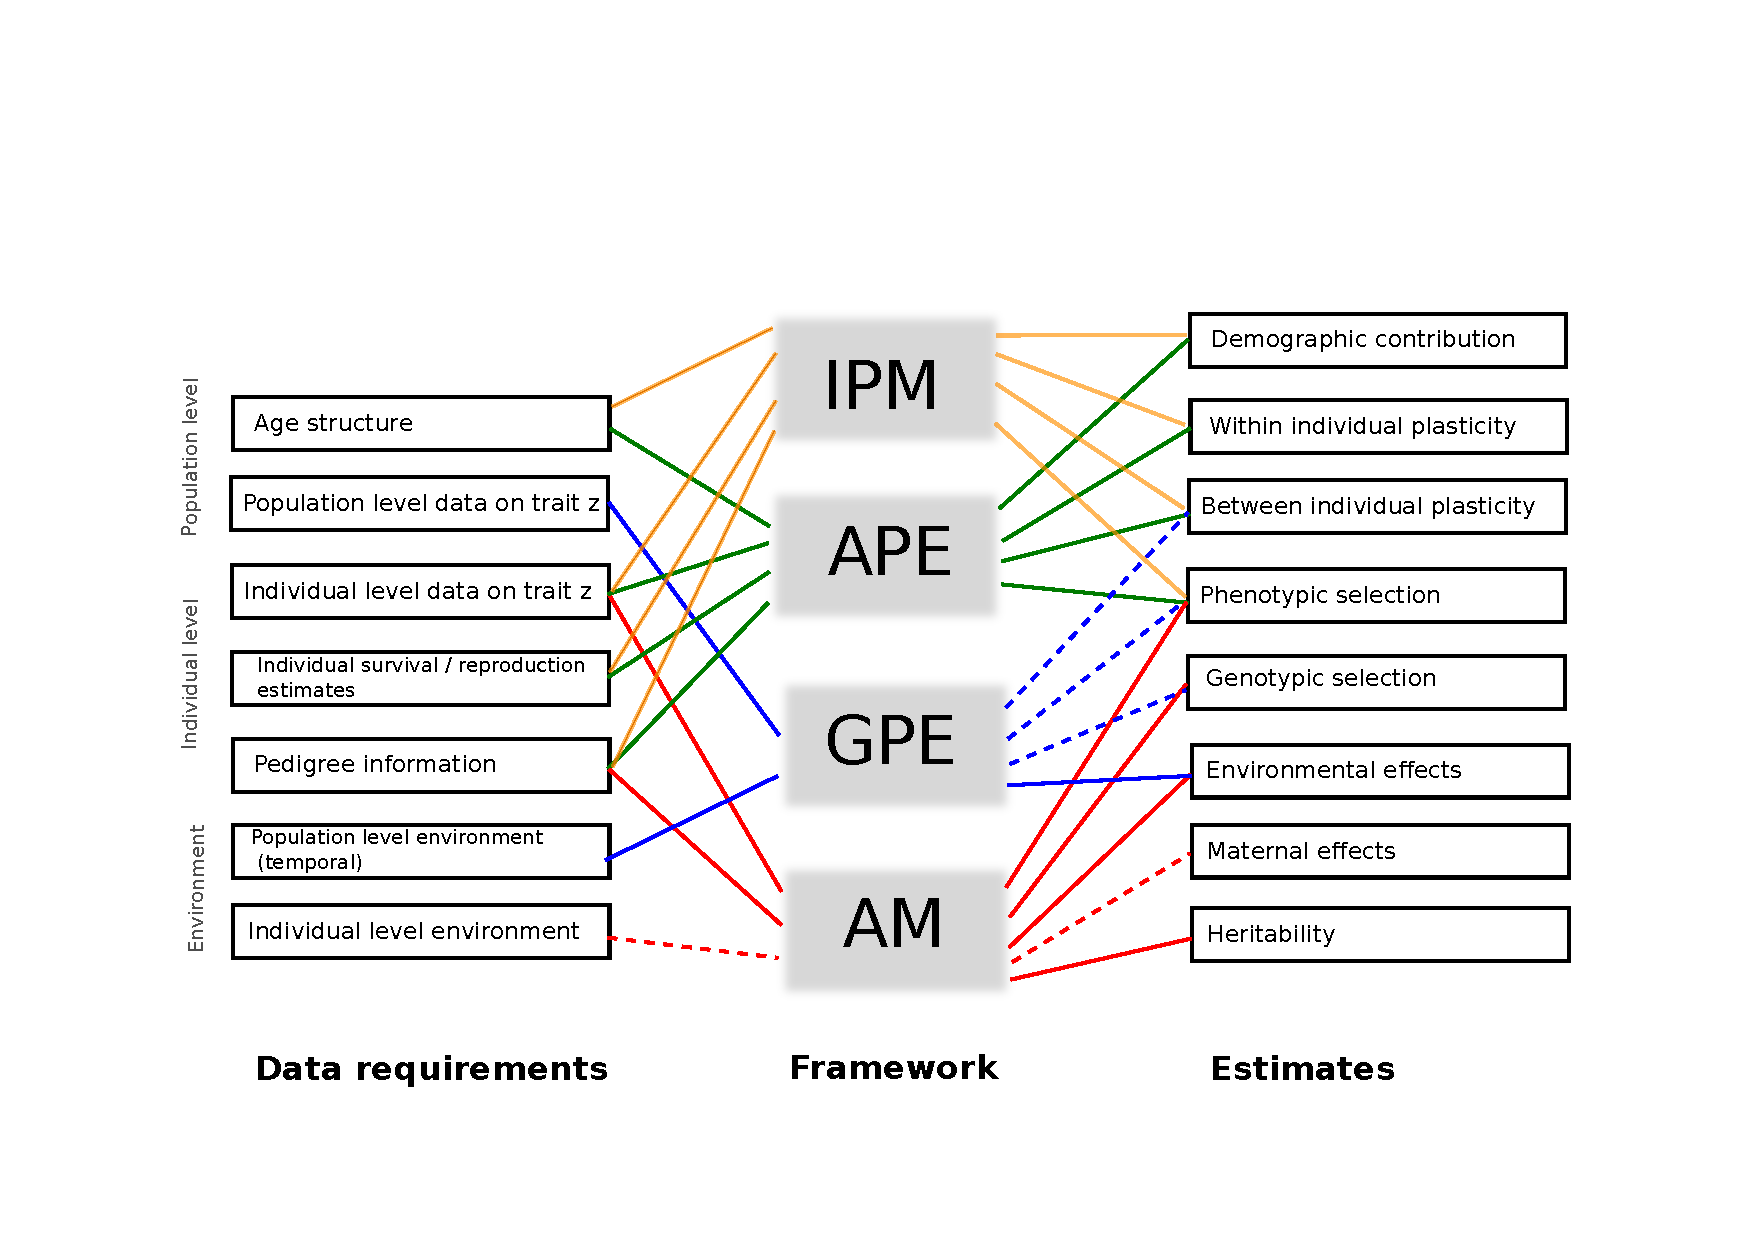
\includegraphics[width=0.85\textwidth]{FiguresDecPop/FigureOverview}
%\caption{Schematic overview of the differences and similarities between the four frameworks (middle column in grey: IPM = Integral Projection Model, APE = Age-structured Price equation, GM = `Geber' method , AM = Animal Model). The frameworks are connected to their data requirements (left) and the processes they are capable of quantifying (right). Note that in the interest of clarity, we have only depicted the more commonly used links. Solid lines represent obligatory links, whereas dashed lines are optional.}
%\label{overview}
%\end{figure}
%
%\newpage
%
%\begin{figure}
%\begin{tabular}{lll}
%\subfigure[]{
%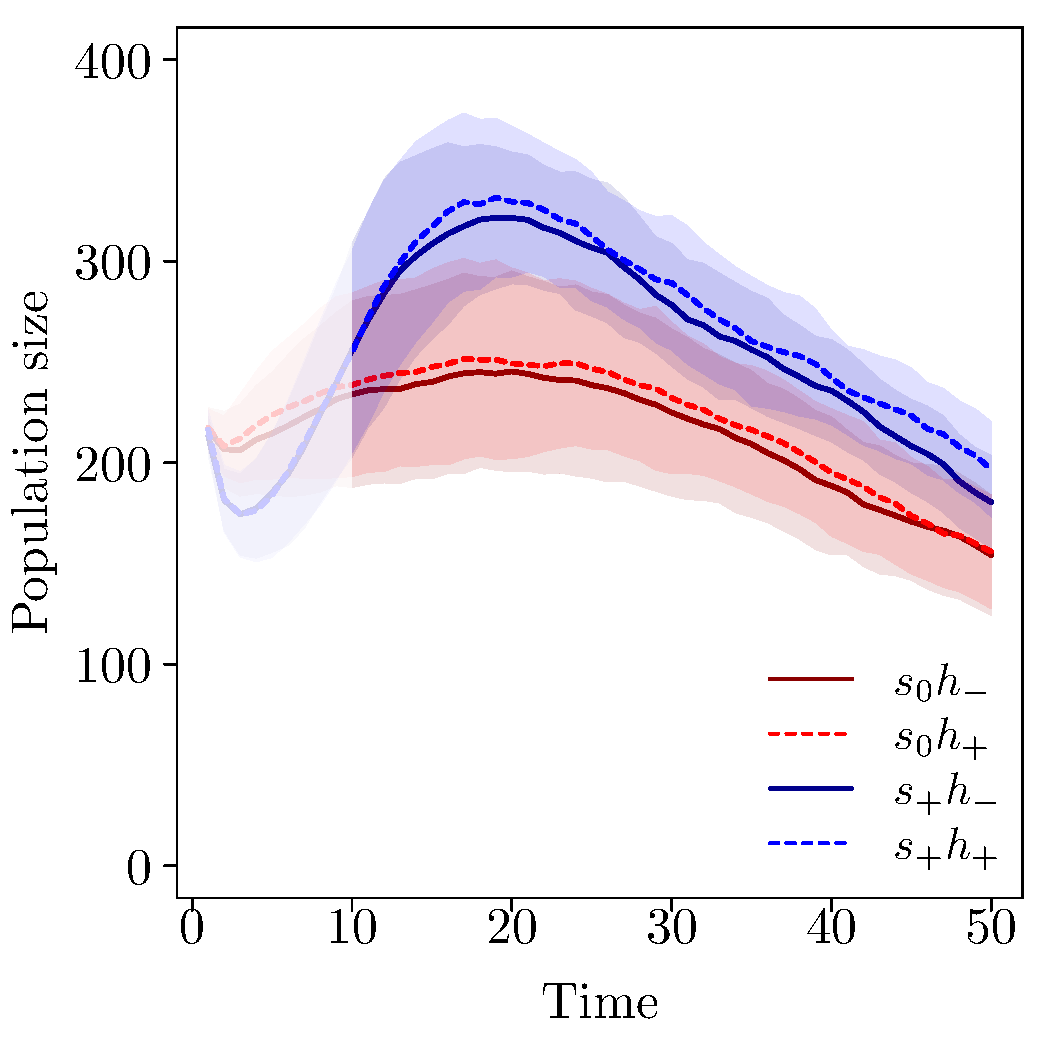
\includegraphics[width=0.3\textwidth]{FiguresDecPop/pop_size}
%\label{simdata:1}
%}
%&
%\subfigure[]{
%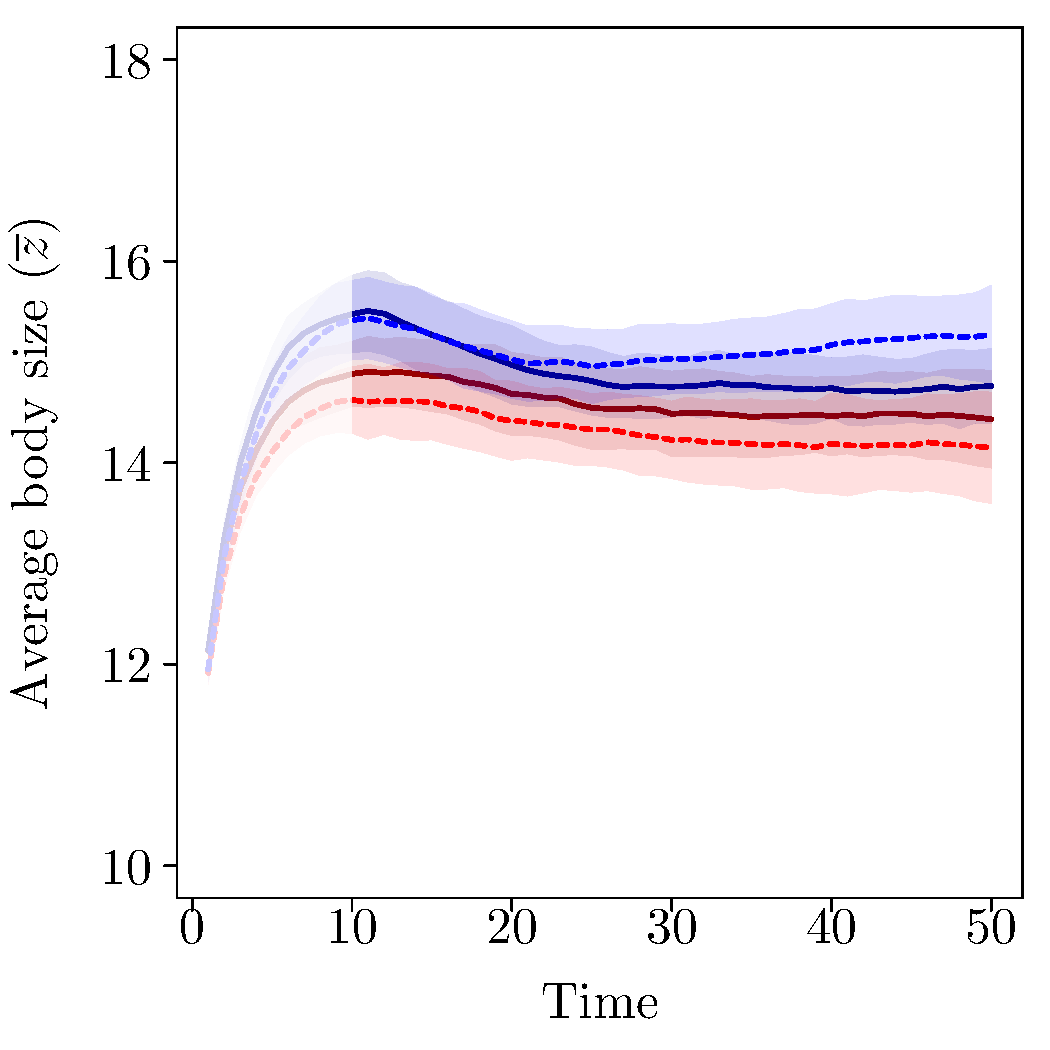
\includegraphics[width=0.3\textwidth]{FiguresDecPop/body_size}
%\label{simdata:2}
%}
%&
%\subfigure[]{
%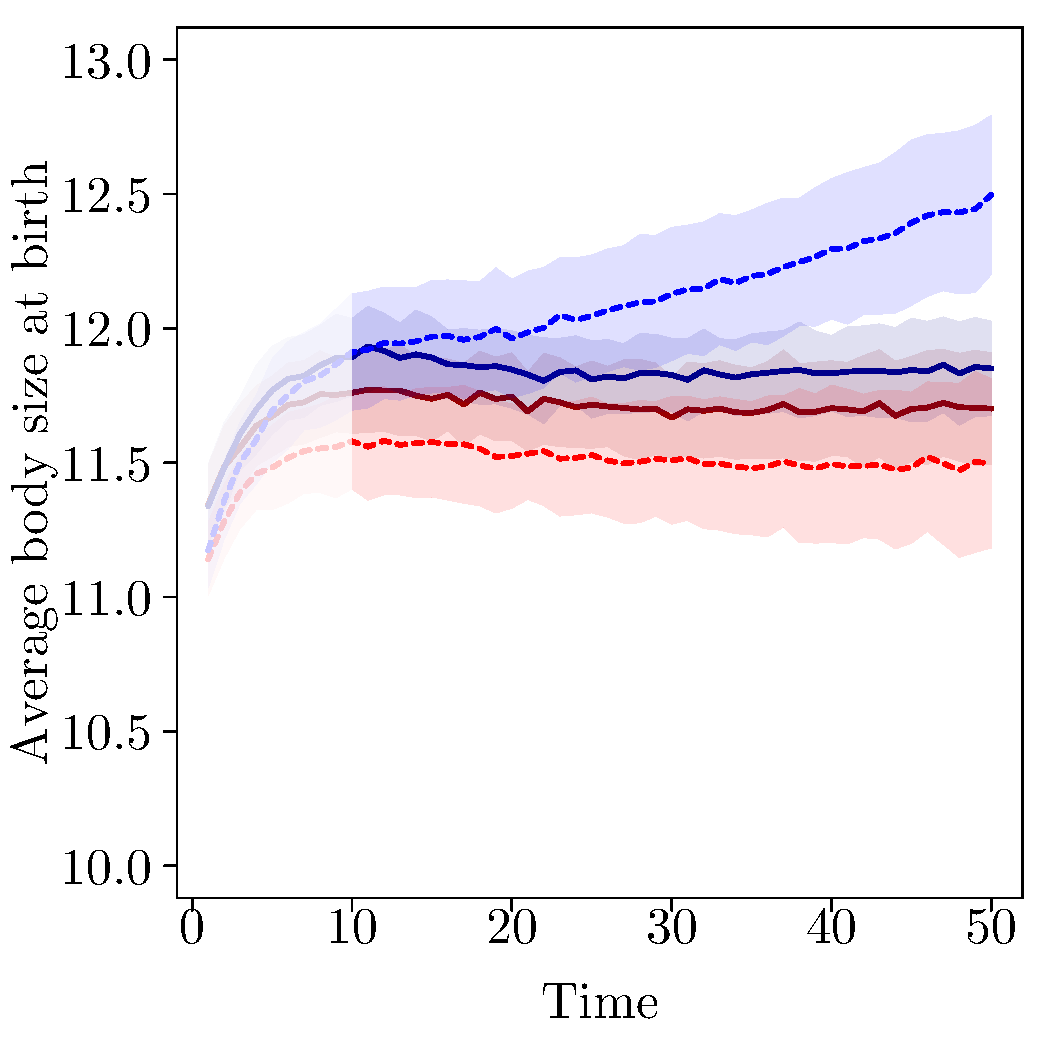
\includegraphics[width=0.3\textwidth]{FiguresDecPop/birth_size}
%\label{simdata:5}
%}
%\\
%\subfigure[]{
%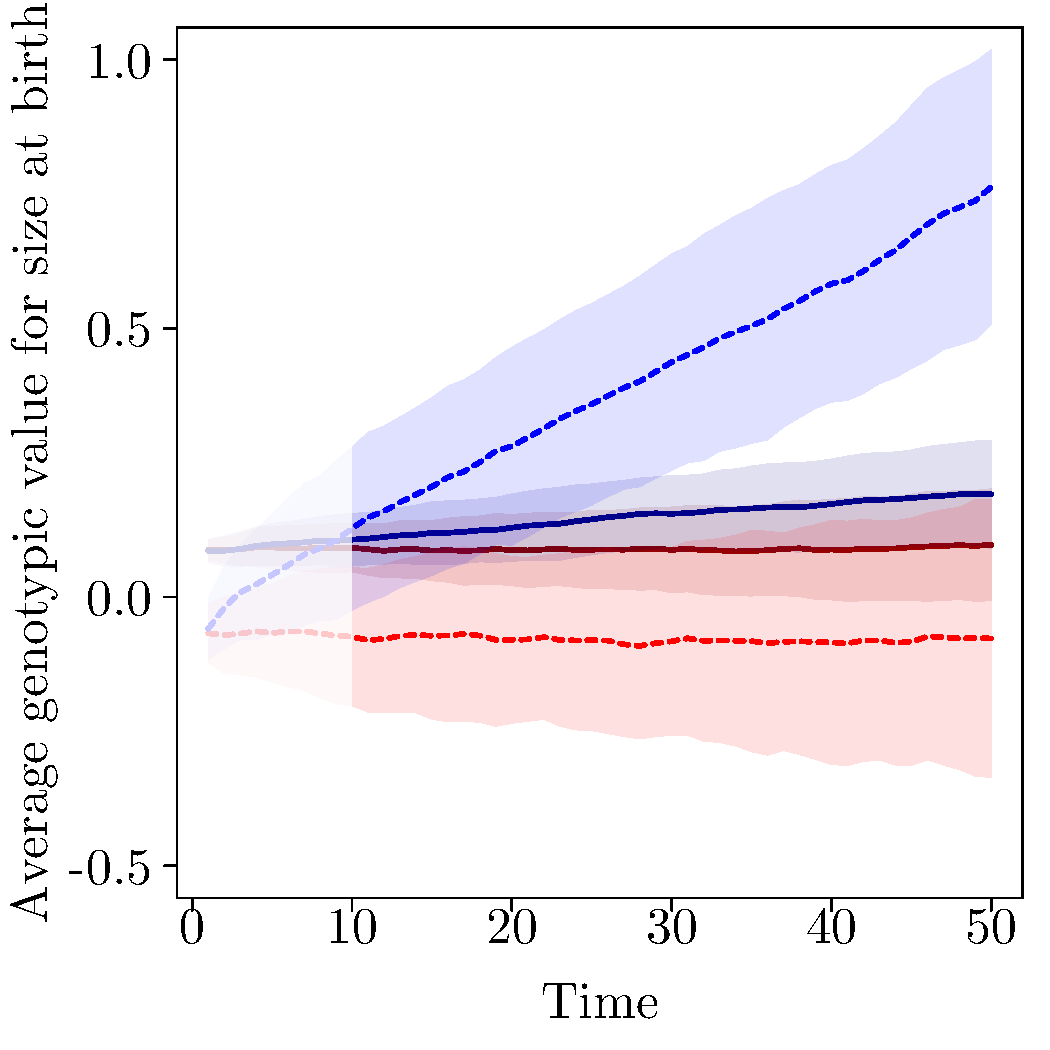
\includegraphics[width=0.3\textwidth]{FiguresDecPop/genotypic_vals}
%\label{simdata:3}
%}
%&
%\subfigure[]{
%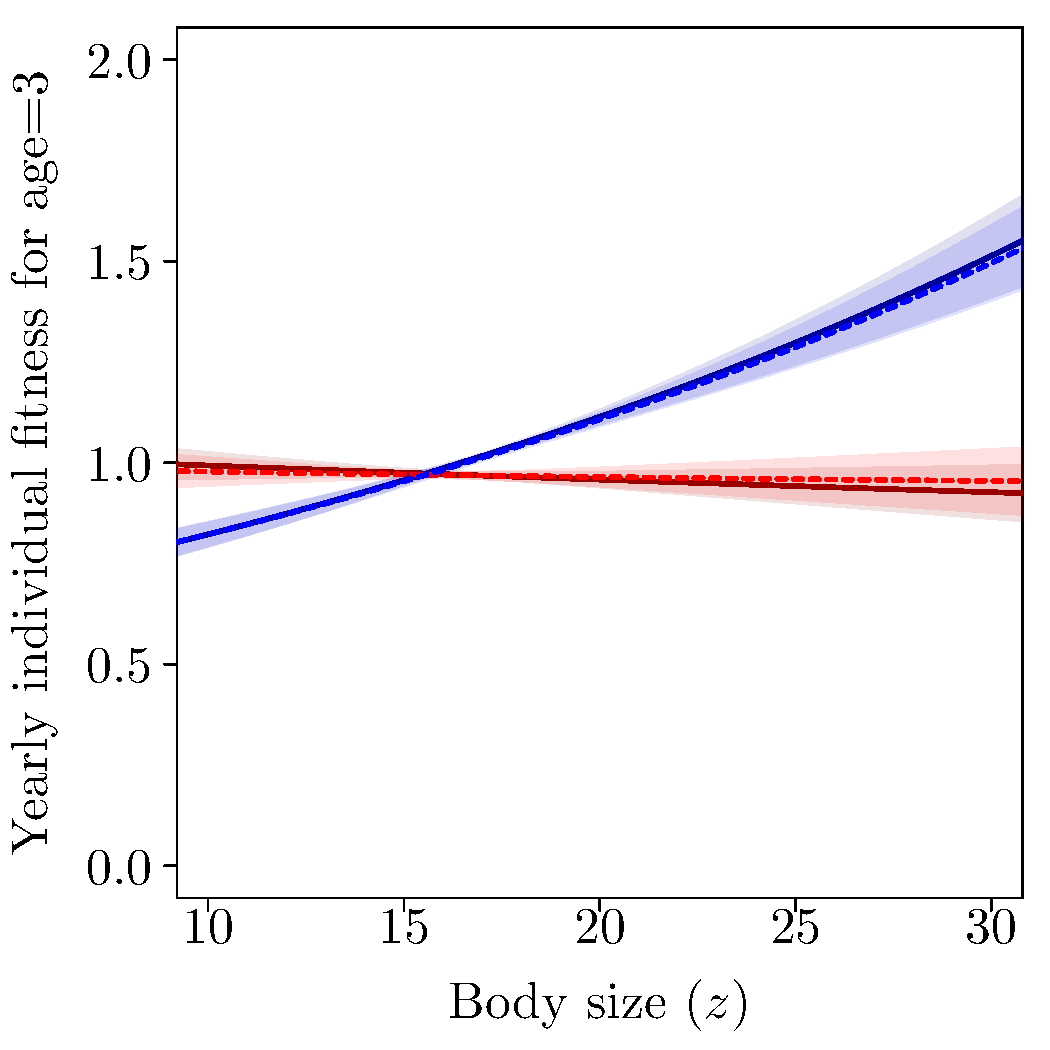
\includegraphics[width=0.3\textwidth]{FiguresDecPop/trait_fitness}
%\label{simdata:4}
%}
%&
%\subfigure[]{
%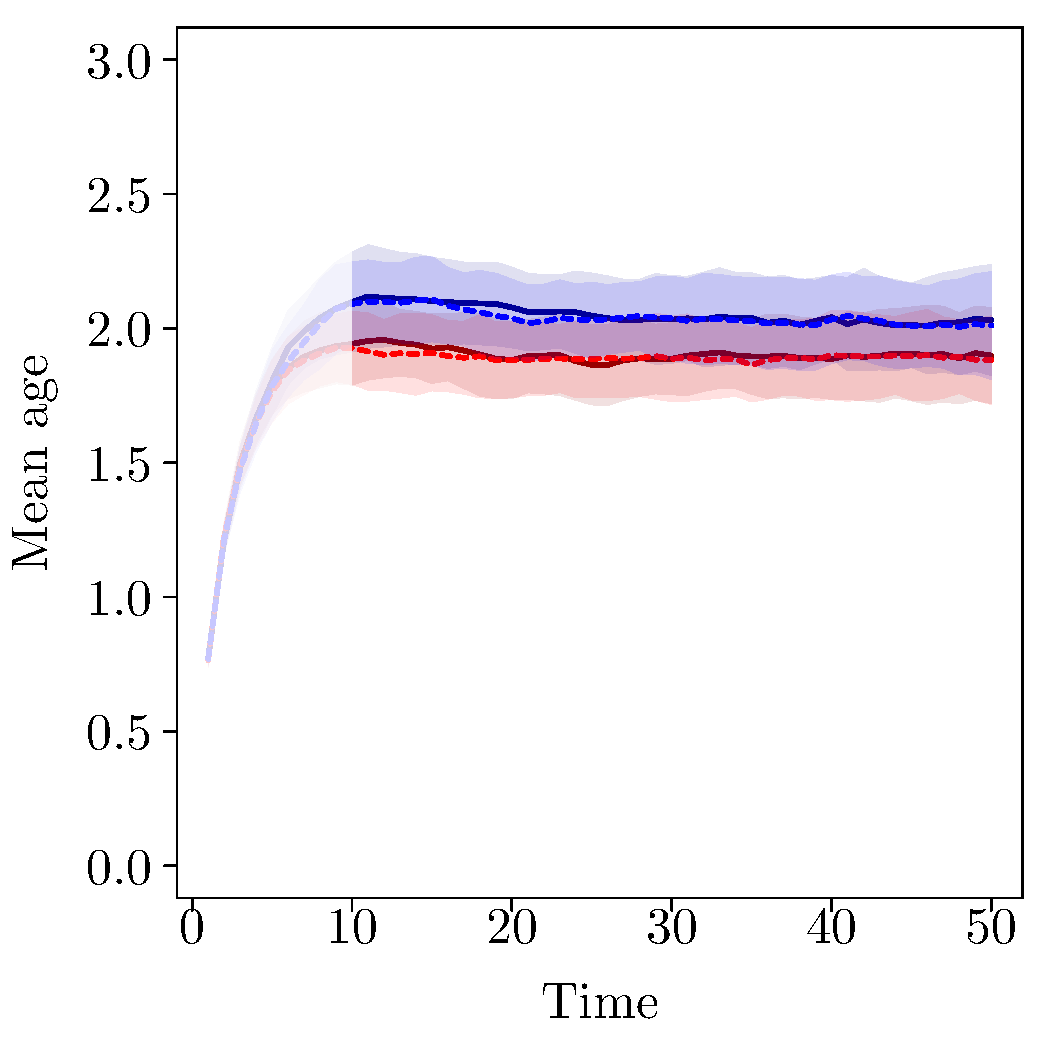
\includegraphics[width=0.3\textwidth]{FiguresDecPop/mean_age}
%\label{simdata:6}
%}
%\end{tabular}
%\caption{Summary of the observed population and trait dynamics of simulated datasets. \subref{simdata:1} Trends in population size, \subref{simdata:2} changes in mean body size, \subref{simdata:5} mean birth size, \subref{simdata:3} and genotypic values for body size, \subref{simdata:4} relations between body size and yearly individual fitness (sum of survival and litter size at $t+1$), and \subref{simdata:6} changes in mean age. Lines indicate the averages across 100 replicates. Polygons show one standard deviation above and below the average. Red lines indicate $s_0$ scenarios (no viability and fertility selection), blue lines indicate $s_+$scenarios (strong viability and fertility selection). Solid lines indicate $h_{-}$ scenarios (low heritability), dotted lines indicate $h_{+}$ scenarios (high heritability). In a-d and f, the white polygon indicates the first 10 years, which are excluded from further analysis. In e, lines are averaged predictions based on generalized additive models over all replicates.}
%\label{simdata}
%\end{figure}
%
%\newpage
%
%\begin{figure}
%\subfigure[]{
%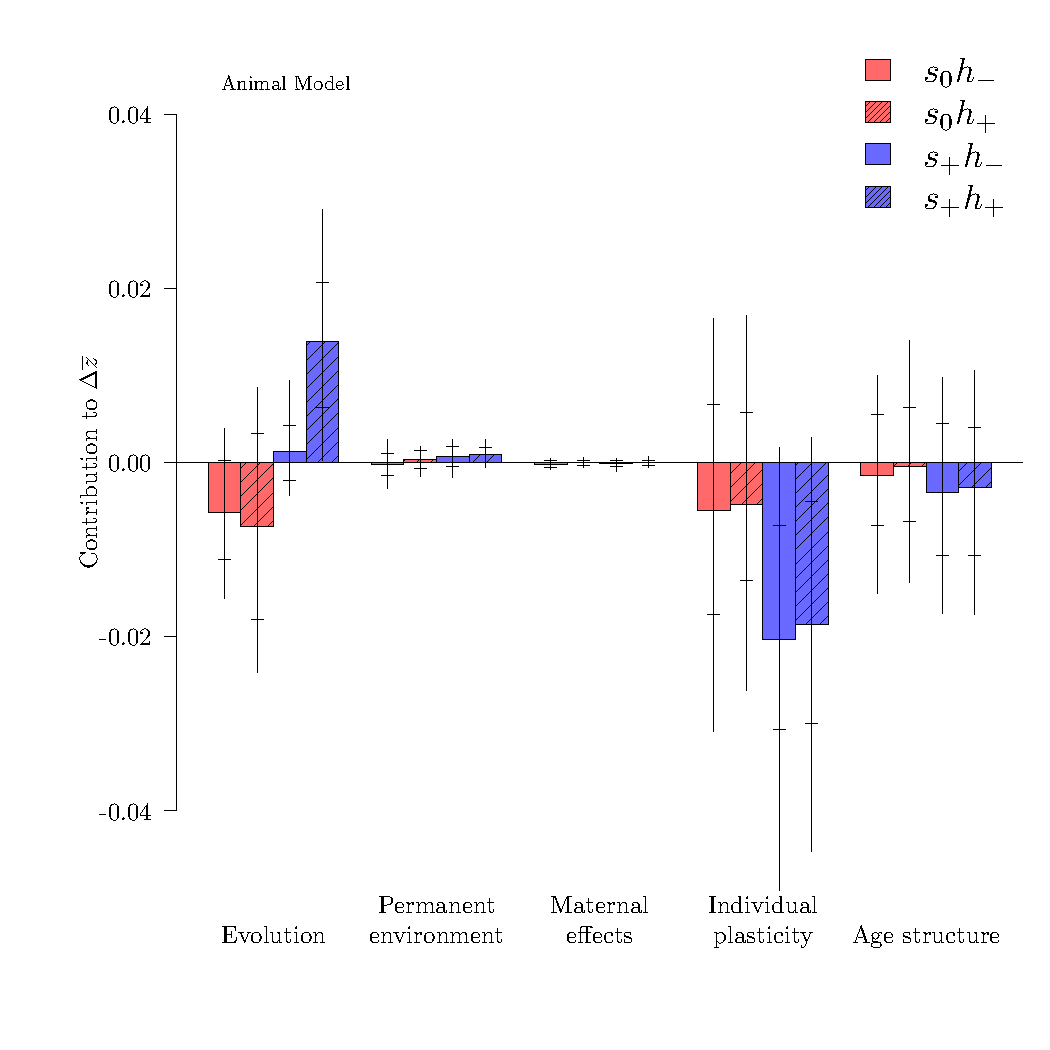
\includegraphics[width=0.5\textwidth]{FiguresDecPop/AM_res}
%\label{frameworkresults:2}
%}
%\subfigure[]{
%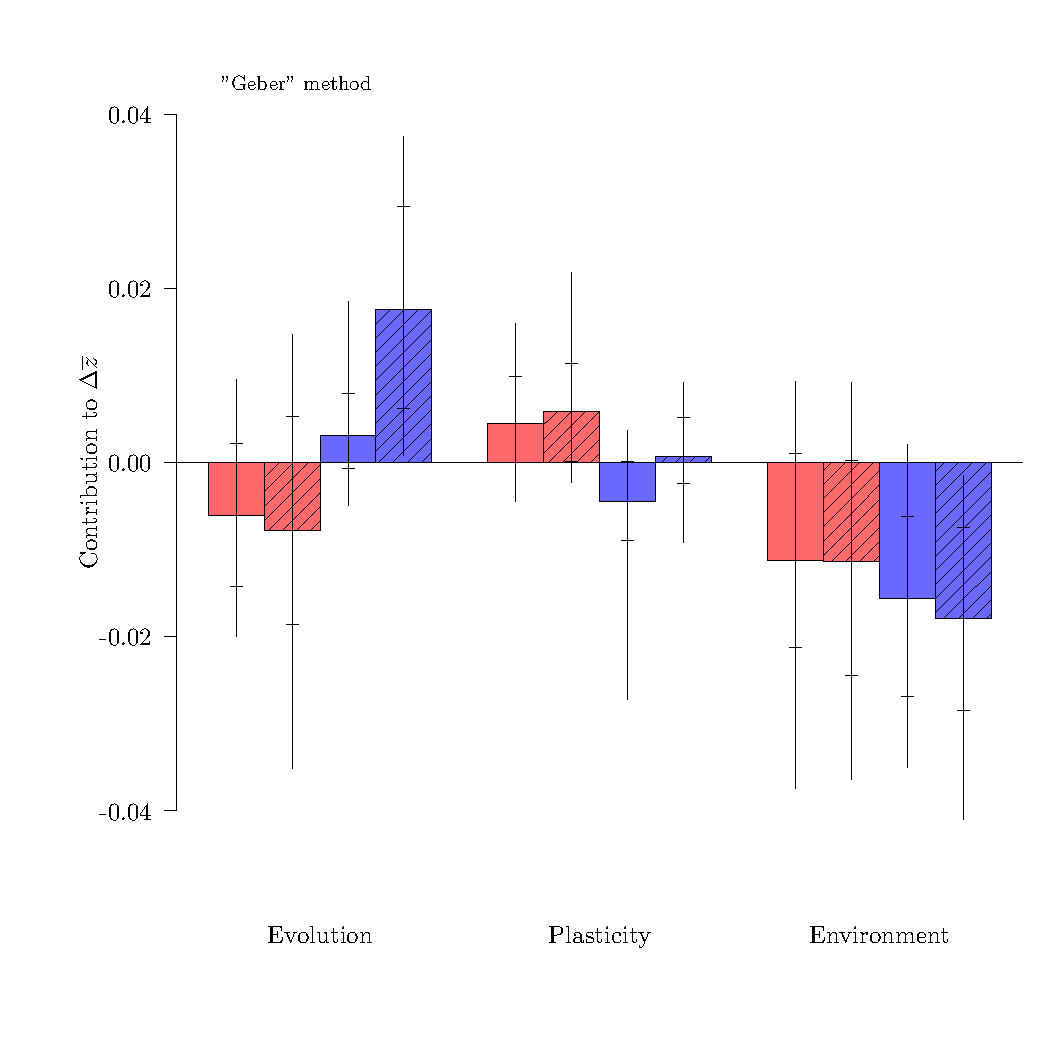
\includegraphics[width=0.5\textwidth]{FiguresDecPop/GPE_res}
%\label{frameworkresults:3}
%}\\
%\subfigure[]{
%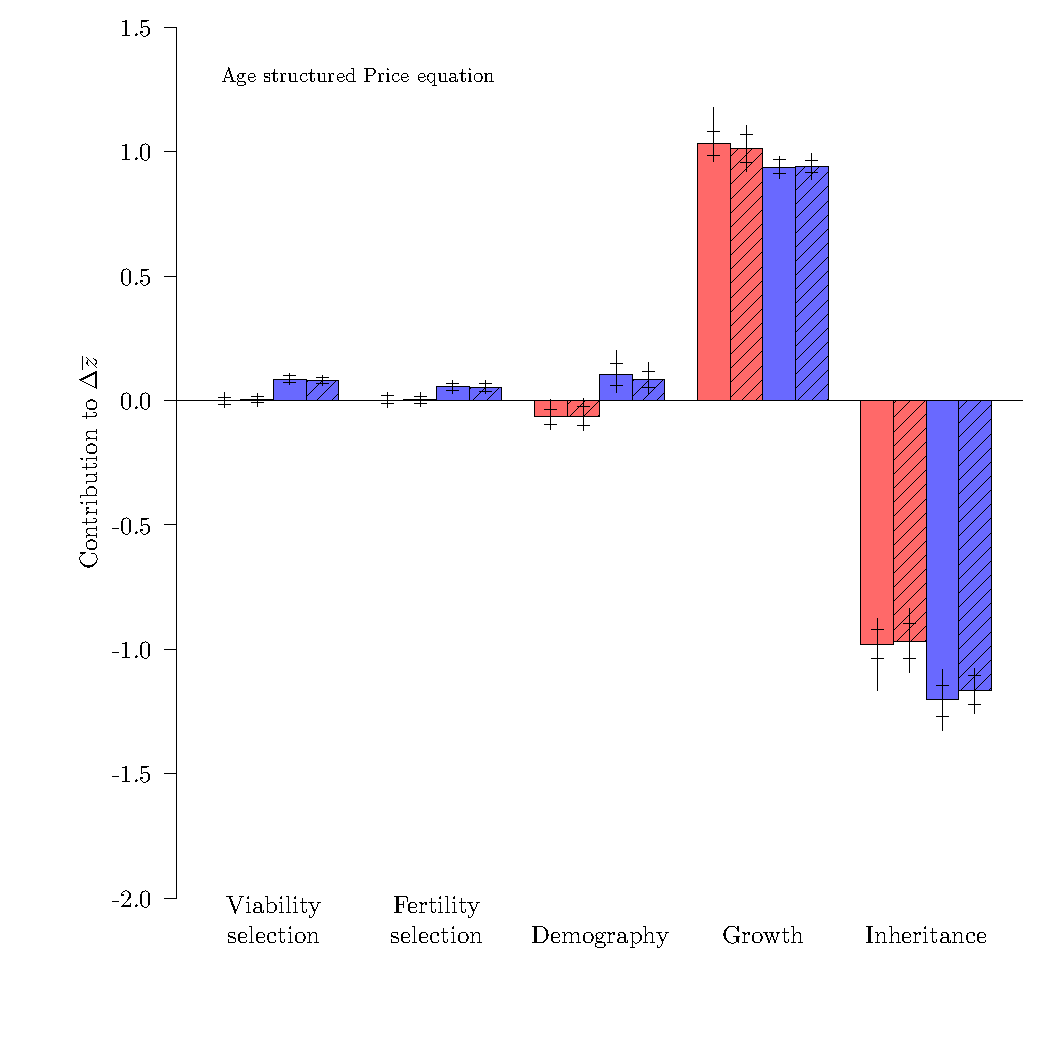
\includegraphics[width=0.5\textwidth]{FiguresDecPop/APE_res}
%\label{frameworkresults:1}
%}
%\subfigure[]{
%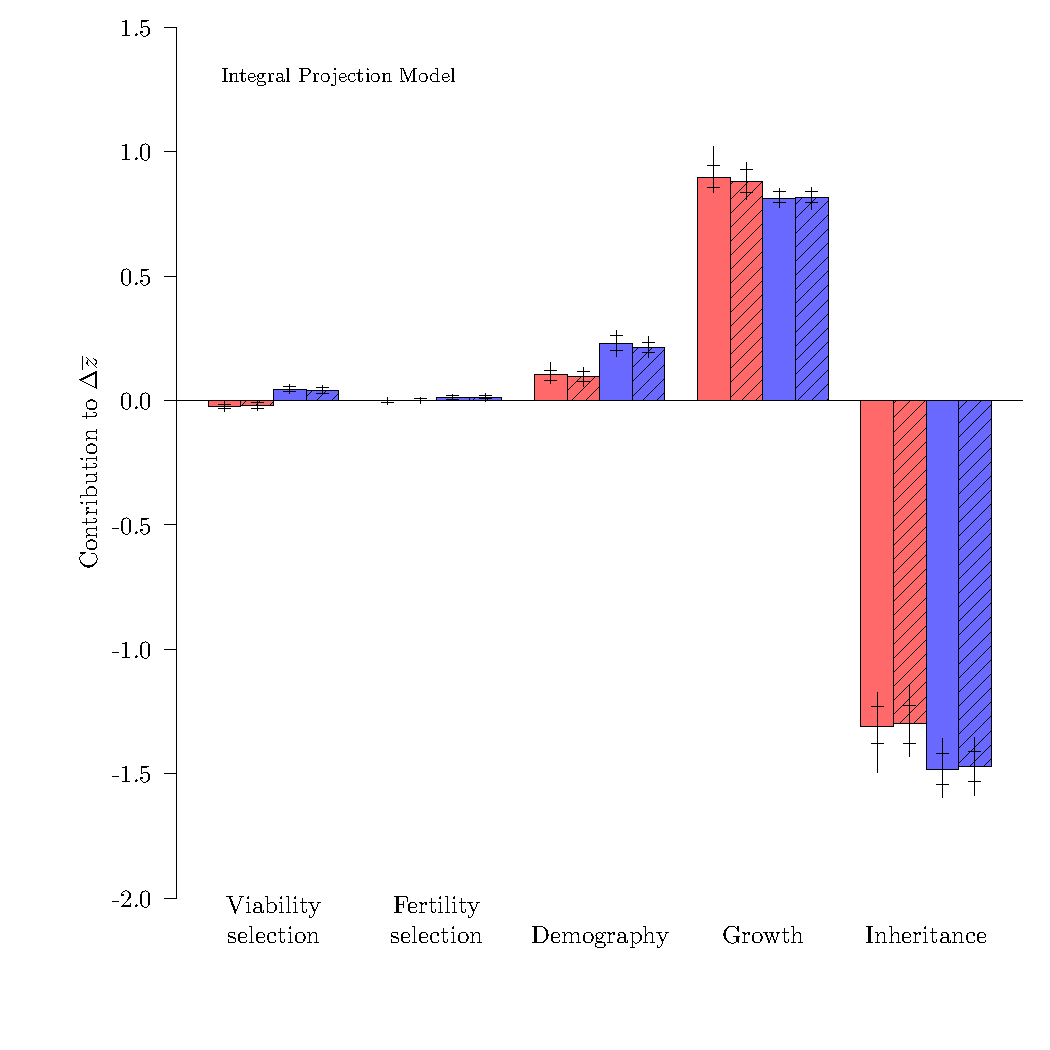
\includegraphics[width=0.5\textwidth]{FiguresDecPop/IPM_res}
%\label{frameworkresults:4}
%}
%
%\caption{Results of the different frameworks when applied to the simulated scenarios. \subref{frameworkresults:2} Animal model. \subref{frameworkresults:3} "Geber" method. \subref{frameworkresults:1} Age-structured Price equation and \subref{frameworkresults:4} Integral projection model. In \subref{frameworkresults:1} and \subref{frameworkresults:4}, demography includes changes in demographic structure due to mortality and natality, inheritance is the sum of offspring mother difference and offspring difference covariance. In a-d, red bars indicate $s_0$ scenarios, blue bars indicate $s_+$ scenarios. Solid bars indicate $h_{-}$ scenarios, and shaded bars indicate $h_{+}$ scenarios. Error bars represent the range in which 68\% (error bars until horizontal lines) and 95\% (entire error bars) of the contributions lie when applied to 100 replicates. Note the different scale on the y-axis in a, b versus c, d.}
%\label{frameworkresults}
%\end{figure}

%%%%%%%%%%%%%%%%%%%%%%%%%%%%%%%%%%%%%%%%%%%%%%%%%%%%%%%%%%%%%%%%%%%%%%%%%%%%%%

\printbibliography[heading=subbibliography]

\newpage
\textbf{\LARGE{Supplementary information}}